\documentclass[]{article}
\usepackage{lmodern}
\usepackage{amssymb,amsmath}
\usepackage{ifxetex,ifluatex}
\usepackage{fixltx2e} % provides \textsubscript
\ifnum 0\ifxetex 1\fi\ifluatex 1\fi=0 % if pdftex
  \usepackage[T1]{fontenc}
  \usepackage[utf8]{inputenc}
\else % if luatex or xelatex
  \ifxetex
    \usepackage{mathspec}
  \else
    \usepackage{fontspec}
  \fi
  \defaultfontfeatures{Ligatures=TeX,Scale=MatchLowercase}
\fi
% use upquote if available, for straight quotes in verbatim environments
\IfFileExists{upquote.sty}{\usepackage{upquote}}{}
% use microtype if available
\IfFileExists{microtype.sty}{%
\usepackage{microtype}
\UseMicrotypeSet[protrusion]{basicmath} % disable protrusion for tt fonts
}{}
\usepackage[margin=1in]{geometry}
\usepackage{hyperref}
\hypersetup{unicode=true,
            pdftitle={project5\_4},
            pdfborder={0 0 0},
            breaklinks=true}
\urlstyle{same}  % don't use monospace font for urls
\usepackage{color}
\usepackage{fancyvrb}
\newcommand{\VerbBar}{|}
\newcommand{\VERB}{\Verb[commandchars=\\\{\}]}
\DefineVerbatimEnvironment{Highlighting}{Verbatim}{commandchars=\\\{\}}
% Add ',fontsize=\small' for more characters per line
\usepackage{framed}
\definecolor{shadecolor}{RGB}{248,248,248}
\newenvironment{Shaded}{\begin{snugshade}}{\end{snugshade}}
\newcommand{\KeywordTok}[1]{\textcolor[rgb]{0.13,0.29,0.53}{\textbf{#1}}}
\newcommand{\DataTypeTok}[1]{\textcolor[rgb]{0.13,0.29,0.53}{#1}}
\newcommand{\DecValTok}[1]{\textcolor[rgb]{0.00,0.00,0.81}{#1}}
\newcommand{\BaseNTok}[1]{\textcolor[rgb]{0.00,0.00,0.81}{#1}}
\newcommand{\FloatTok}[1]{\textcolor[rgb]{0.00,0.00,0.81}{#1}}
\newcommand{\ConstantTok}[1]{\textcolor[rgb]{0.00,0.00,0.00}{#1}}
\newcommand{\CharTok}[1]{\textcolor[rgb]{0.31,0.60,0.02}{#1}}
\newcommand{\SpecialCharTok}[1]{\textcolor[rgb]{0.00,0.00,0.00}{#1}}
\newcommand{\StringTok}[1]{\textcolor[rgb]{0.31,0.60,0.02}{#1}}
\newcommand{\VerbatimStringTok}[1]{\textcolor[rgb]{0.31,0.60,0.02}{#1}}
\newcommand{\SpecialStringTok}[1]{\textcolor[rgb]{0.31,0.60,0.02}{#1}}
\newcommand{\ImportTok}[1]{#1}
\newcommand{\CommentTok}[1]{\textcolor[rgb]{0.56,0.35,0.01}{\textit{#1}}}
\newcommand{\DocumentationTok}[1]{\textcolor[rgb]{0.56,0.35,0.01}{\textbf{\textit{#1}}}}
\newcommand{\AnnotationTok}[1]{\textcolor[rgb]{0.56,0.35,0.01}{\textbf{\textit{#1}}}}
\newcommand{\CommentVarTok}[1]{\textcolor[rgb]{0.56,0.35,0.01}{\textbf{\textit{#1}}}}
\newcommand{\OtherTok}[1]{\textcolor[rgb]{0.56,0.35,0.01}{#1}}
\newcommand{\FunctionTok}[1]{\textcolor[rgb]{0.00,0.00,0.00}{#1}}
\newcommand{\VariableTok}[1]{\textcolor[rgb]{0.00,0.00,0.00}{#1}}
\newcommand{\ControlFlowTok}[1]{\textcolor[rgb]{0.13,0.29,0.53}{\textbf{#1}}}
\newcommand{\OperatorTok}[1]{\textcolor[rgb]{0.81,0.36,0.00}{\textbf{#1}}}
\newcommand{\BuiltInTok}[1]{#1}
\newcommand{\ExtensionTok}[1]{#1}
\newcommand{\PreprocessorTok}[1]{\textcolor[rgb]{0.56,0.35,0.01}{\textit{#1}}}
\newcommand{\AttributeTok}[1]{\textcolor[rgb]{0.77,0.63,0.00}{#1}}
\newcommand{\RegionMarkerTok}[1]{#1}
\newcommand{\InformationTok}[1]{\textcolor[rgb]{0.56,0.35,0.01}{\textbf{\textit{#1}}}}
\newcommand{\WarningTok}[1]{\textcolor[rgb]{0.56,0.35,0.01}{\textbf{\textit{#1}}}}
\newcommand{\AlertTok}[1]{\textcolor[rgb]{0.94,0.16,0.16}{#1}}
\newcommand{\ErrorTok}[1]{\textcolor[rgb]{0.64,0.00,0.00}{\textbf{#1}}}
\newcommand{\NormalTok}[1]{#1}
\usepackage{graphicx,grffile}
\makeatletter
\def\maxwidth{\ifdim\Gin@nat@width>\linewidth\linewidth\else\Gin@nat@width\fi}
\def\maxheight{\ifdim\Gin@nat@height>\textheight\textheight\else\Gin@nat@height\fi}
\makeatother
% Scale images if necessary, so that they will not overflow the page
% margins by default, and it is still possible to overwrite the defaults
% using explicit options in \includegraphics[width, height, ...]{}
\setkeys{Gin}{width=\maxwidth,height=\maxheight,keepaspectratio}
\IfFileExists{parskip.sty}{%
\usepackage{parskip}
}{% else
\setlength{\parindent}{0pt}
\setlength{\parskip}{6pt plus 2pt minus 1pt}
}
\setlength{\emergencystretch}{3em}  % prevent overfull lines
\providecommand{\tightlist}{%
  \setlength{\itemsep}{0pt}\setlength{\parskip}{0pt}}
\setcounter{secnumdepth}{0}
% Redefines (sub)paragraphs to behave more like sections
\ifx\paragraph\undefined\else
\let\oldparagraph\paragraph
\renewcommand{\paragraph}[1]{\oldparagraph{#1}\mbox{}}
\fi
\ifx\subparagraph\undefined\else
\let\oldsubparagraph\subparagraph
\renewcommand{\subparagraph}[1]{\oldsubparagraph{#1}\mbox{}}
\fi

%%% Use protect on footnotes to avoid problems with footnotes in titles
\let\rmarkdownfootnote\footnote%
\def\footnote{\protect\rmarkdownfootnote}

%%% Change title format to be more compact
\usepackage{titling}

% Create subtitle command for use in maketitle
\newcommand{\subtitle}[1]{
  \posttitle{
    \begin{center}\large#1\end{center}
    }
}

\setlength{\droptitle}{-2em}
  \title{project5\_4}
  \pretitle{\vspace{\droptitle}\centering\huge}
  \posttitle{\par}
  \author{}
  \preauthor{}\postauthor{}
  \date{}
  \predate{}\postdate{}


\begin{document}
\maketitle

\subsection{Introduction}\label{introduction}

This Project aims to explore which type of severe event can cause most
fatalities, injuries, property damage or crop damge.\\
The raw dataset is obtained from
\href{https://d396qusza40orc.cloudfront.net/repdata\%2Fdata\%2FStormData.csv.bz2}{U.S.
National Oceanic and Atmospheric Administration's (NOAA) storm database}
which contains a series of events with recorded fatalies, injuries,
property damages and so on from 1950 to November 2011.

In this particular project, we only forcus on fatalities, injuries,
property damage and crop damage, which is the reason why we only select
those columns from the dataset.

To find which types of events (as indicated in the 𝙴𝚅𝚃𝚈𝙿𝙴 variable) are
most harmful with respect to population health, we have tried two
different approaches: 1. Rank the harmfulness primarily by
``FATALITIES'' then ``INJURIES'' due to the fact that fatalities is
considered more servere.\\
2. Rank the harmfulness by the sum of ``FATALITIES'' and ``INJURIES''.

To find which types of events have the greatest economic consequences,
we simply examin the total damage caused, which is evaluated by dollars.

The panel graphs are drawn to show the comparison with all R codes
provided for the purpose of reproducibility.

\subsection{Data Processing}\label{data-processing}

Firstly, we need to set up the enviroment correctly with the following
code:

\begin{Shaded}
\begin{Highlighting}[]
\KeywordTok{setwd}\NormalTok{(}\StringTok{"~/Desktop/Coursera Datascience"}\NormalTok{)}
\KeywordTok{rm}\NormalTok{(}\DataTypeTok{list =} \KeywordTok{ls}\NormalTok{())}
\KeywordTok{library}\NormalTok{(ggplot2)}
\KeywordTok{library}\NormalTok{(reshape2)}
\KeywordTok{library}\NormalTok{(gridExtra)}
\ControlFlowTok{if}\NormalTok{ (}\OperatorTok{!}\KeywordTok{file.exists}\NormalTok{(}\StringTok{"./wk5_4"}\NormalTok{)) \{}\KeywordTok{dir.create}\NormalTok{(}\StringTok{"./wk5_4"}\NormalTok{)\}}
\end{Highlighting}
\end{Shaded}

As mentioned, the raw data is downloaded from
\href{https://d396qusza40orc.cloudfront.net/repdata\%2Fdata\%2FStormData.csv.bz2}{U.S.
National Oceanic and Atmospheric Administration's (NOAA) storm
database}.

\begin{Shaded}
\begin{Highlighting}[]
\ControlFlowTok{if}\NormalTok{ (}\OperatorTok{!}\KeywordTok{file.exists}\NormalTok{(}\StringTok{"./wk5_4/data.bz2"}\NormalTok{))\{}
\NormalTok{  fileurl <-}\StringTok{ "https://d396qusza40orc.cloudfront.net/repdata%2Fdata%2FStormData.csv.bz2"}
  \KeywordTok{download.file}\NormalTok{(fileurl,destfile <-}\StringTok{ "./wk5_4/data.bz2"}\NormalTok{,}\DataTypeTok{method =} \StringTok{"curl"}\NormalTok{,}\DataTypeTok{mode =} \StringTok{"wb"}\NormalTok{)}
\NormalTok{\}}
\NormalTok{  raw_dat <-}\StringTok{ }\KeywordTok{read.csv}\NormalTok{(}\StringTok{"./wk5_4/data.bz2"}\NormalTok{) }
\end{Highlighting}
\end{Shaded}

The preprocessing steps simply scale up the property damages and crop
damages as indicated by the variable \texttt{PROPDMGEXP} and
\texttt{CROPDMGEXP} where {[}Bb{]} represnets 10\^{}9, {[}Mm{]}
represnts 10\^{}6, {[}Kk{]} represents 10\^{}3 and {[}Hh{]} represnts
10\^{}2 respectively.

\begin{Shaded}
\begin{Highlighting}[]
\NormalTok{dat <-}\StringTok{ }\KeywordTok{subset}\NormalTok{(raw_dat,}\DataTypeTok{select =} \KeywordTok{c}\NormalTok{(EVTYPE,FATALITIES,INJURIES,PROPDMG,PROPDMGEXP,CROPDMG,CROPDMGEXP))}
\NormalTok{kindexp <-}\StringTok{ }\NormalTok{dat}\OperatorTok{$}\NormalTok{PROPDMGEXP }\OperatorTok{==}\StringTok{ "K"}
\NormalTok{bindexp <-}\StringTok{ }\NormalTok{dat}\OperatorTok{$}\NormalTok{PROPDMGEXP }\OperatorTok{==}\StringTok{ "B"}
\NormalTok{hindexp <-}\StringTok{ }\NormalTok{dat}\OperatorTok{$}\NormalTok{PROPDMGEXP }\OperatorTok{==}\StringTok{ "h"}\OperatorTok{|}\StringTok{ }\NormalTok{dat}\OperatorTok{$}\NormalTok{PROPDMGEXP }\OperatorTok{==}\StringTok{ "H"}
\NormalTok{mindexp <-}\StringTok{ }\NormalTok{dat}\OperatorTok{$}\NormalTok{PROPDMGEXP }\OperatorTok{==}\StringTok{ "m"}\OperatorTok{|}\StringTok{ }\NormalTok{dat}\OperatorTok{$}\NormalTok{PROPDMGEXP }\OperatorTok{==}\StringTok{ "M"}
\NormalTok{bindexc <-}\StringTok{ }\NormalTok{dat}\OperatorTok{$}\NormalTok{CROPDMGEXP }\OperatorTok{==}\StringTok{ "B"}
\NormalTok{kindexc <-}\StringTok{ }\NormalTok{dat}\OperatorTok{$}\NormalTok{CROPDMGEXP }\OperatorTok{==}\StringTok{ "k"}\OperatorTok{|}\StringTok{ }\NormalTok{dat}\OperatorTok{$}\NormalTok{CROPDMGEXP }\OperatorTok{==}\StringTok{ "K"}
\NormalTok{mindexc <-}\StringTok{ }\NormalTok{dat}\OperatorTok{$}\NormalTok{CROPDMGEXP }\OperatorTok{==}\StringTok{ "m"}\OperatorTok{|}\StringTok{ }\NormalTok{dat}\OperatorTok{$}\NormalTok{CROPDMGEXP }\OperatorTok{==}\StringTok{ "M"}
\NormalTok{dat}\OperatorTok{$}\NormalTok{PROPDMG[kindexp] <-}\StringTok{ }\NormalTok{dat}\OperatorTok{$}\NormalTok{PROPDMG[kindexp]}\OperatorTok{*}\DecValTok{10}\OperatorTok{^}\DecValTok{3}
\NormalTok{dat}\OperatorTok{$}\NormalTok{PROPDMG[bindexp] <-}\StringTok{ }\NormalTok{dat}\OperatorTok{$}\NormalTok{PROPDMG[bindexp]}\OperatorTok{*}\DecValTok{10}\OperatorTok{^}\DecValTok{9}
\NormalTok{dat}\OperatorTok{$}\NormalTok{PROPDMG[hindexp] <-}\StringTok{ }\NormalTok{dat}\OperatorTok{$}\NormalTok{PROPDMG[hindexp]}\OperatorTok{*}\DecValTok{10}\OperatorTok{^}\DecValTok{2}
\NormalTok{dat}\OperatorTok{$}\NormalTok{PROPDMG[mindexp] <-}\StringTok{ }\NormalTok{dat}\OperatorTok{$}\NormalTok{PROPDMG[mindexp]}\OperatorTok{*}\DecValTok{10}\OperatorTok{^}\DecValTok{6}
\NormalTok{dat}\OperatorTok{$}\NormalTok{CROPDMG[bindexc] <-}\StringTok{ }\NormalTok{dat}\OperatorTok{$}\NormalTok{CROPDMG[bindexc]}\OperatorTok{*}\DecValTok{10}\OperatorTok{^}\DecValTok{9}
\NormalTok{dat}\OperatorTok{$}\NormalTok{CROPDMG[kindexc] <-}\StringTok{ }\NormalTok{dat}\OperatorTok{$}\NormalTok{CROPDMG[kindexc]}\OperatorTok{*}\DecValTok{10}\OperatorTok{^}\DecValTok{3}
\NormalTok{dat}\OperatorTok{$}\NormalTok{CROPDMG[mindexc] <-}\StringTok{ }\NormalTok{dat}\OperatorTok{$}\NormalTok{CROPDMG[mindexc]}\OperatorTok{*}\DecValTok{10}\OperatorTok{^}\DecValTok{6}
\NormalTok{tdat <-}\StringTok{ }\KeywordTok{subset}\NormalTok{(dat,}\DataTypeTok{select =} \KeywordTok{c}\NormalTok{(EVTYPE,FATALITIES,INJURIES,PROPDMG,CROPDMG))}
\end{Highlighting}
\end{Shaded}

Order the dataset based on what we are intested at.

\begin{Shaded}
\begin{Highlighting}[]
\NormalTok{bytype <-}\StringTok{ }\KeywordTok{aggregate}\NormalTok{(}\KeywordTok{cbind}\NormalTok{(FATALITIES,INJURIES,}\DataTypeTok{HARMFUL =}\NormalTok{ FATALITIES }\OperatorTok{+}\StringTok{ }\NormalTok{INJURIES,PROPDMG,CROPDMG,}\DataTypeTok{ECODMG =}\NormalTok{ PROPDMG}\OperatorTok{+}\NormalTok{CROPDMG)}\OperatorTok{~}\NormalTok{EVTYPE,tdat,sum)}
\NormalTok{RankFatality <-}\StringTok{ }\NormalTok{bytype[}\KeywordTok{order}\NormalTok{(bytype}\OperatorTok{$}\NormalTok{FATALITIES,}\DataTypeTok{decreasing =} \OtherTok{TRUE}\NormalTok{),]}
\NormalTok{RankInjury <-}\StringTok{ }\NormalTok{bytype[}\KeywordTok{order}\NormalTok{(bytype}\OperatorTok{$}\NormalTok{INJURIES,}\DataTypeTok{decreasing =} \OtherTok{TRUE}\NormalTok{),]}
\NormalTok{RankHarmful1 <-}\StringTok{ }\NormalTok{bytype[}\KeywordTok{order}\NormalTok{(bytype}\OperatorTok{$}\NormalTok{FATALITIES,bytype}\OperatorTok{$}\NormalTok{INJURIES,}\DataTypeTok{decreasing =} \OtherTok{TRUE}\NormalTok{),]}
\NormalTok{RankHarmful2 <-}\StringTok{ }\NormalTok{bytype[}\KeywordTok{order}\NormalTok{(bytype}\OperatorTok{$}\NormalTok{HARMFUL,}\DataTypeTok{decreasing =} \OtherTok{TRUE}\NormalTok{),]}
\NormalTok{RankPropDmg <-}\StringTok{ }\NormalTok{bytype[}\KeywordTok{order}\NormalTok{(bytype}\OperatorTok{$}\NormalTok{PROPDMG,}\DataTypeTok{decreasing =} \OtherTok{TRUE}\NormalTok{),]}
\NormalTok{RankCropDmg <-}\StringTok{ }\NormalTok{bytype[}\KeywordTok{order}\NormalTok{(bytype}\OperatorTok{$}\NormalTok{CROPDMG,}\DataTypeTok{decreasing =} \OtherTok{TRUE}\NormalTok{),]}
\NormalTok{RankEcoDmg <-}\StringTok{ }\NormalTok{bytype[}\KeywordTok{order}\NormalTok{(bytype}\OperatorTok{$}\NormalTok{ECODMG,}\DataTypeTok{decreasing =} \OtherTok{TRUE}\NormalTok{),]}
\end{Highlighting}
\end{Shaded}

\subsection{Results}\label{results}

Here is the results:
\texttt{\{r\ plotHarmful,\ fig.-\ ggplot(data\ =\ RankFatality{[}1:5,{]},\ aes(x\ =\ reorder(EVTYPE,-FATALITIES),\ y\ =\ FATALITIES))\ +\ geom\_bar(stat\ =\ "identity")\ +\ xlab("Event\ Type")\ +\ ylab("\#\ of\ Fatalities")\ p2\ \textless{}-\ ggplot(data\ =\ RankInjury{[}1:5,{]},\ aes(x\ =\ reorder(EVTYPE,-INJURIES),\ y\ =\ INJURIES))\ +\ geom\_bar(stat\ =\ "identity")\ +xlab("Event\ Type")\ +\ ylab("\#\ of\ Injuries")\ TopHarmful1\ \textless{}-\ melt(subset(RankHarmful1{[}1:5,{]},select=c(EVTYPE,FATALITIES,INJURIES)),value.name\ =\ c("value"),variable.name\ =\ "Type")\ p3\ \textless{}-\ ggplot(data\ =\ TopHarmful1,\ aes(x\ =\ reorder(EVTYPE,-TopHarmful1\$value),\ y\ =\ TopHarmful1\$value,fill\ =\ TopHarmful1\$Type))\ +\ geom\_bar(stat\ =\ "identity")\ +xlab("Event\ Type")+\ ylab("\#\ of\ Harmed")\ TopHarmful2\ \textless{}-\ melt(subset(RankHarmful2{[}1:5,{]},select=c(EVTYPE,FATALITIES,INJURIES)),value.name\ =\ c("value"),variable.name\ =\ "Type")\ p4\ \textless{}-\ ggplot(data\ =\ TopHarmful2,\ aes(x\ =\ reorder(EVTYPE,-TopHarmful2\$value),\ y\ =\ TopHarmful2\$value,fill\ =\ TopHarmful2\$Type))\ +\ geom\_bar(stat\ =\ "identity")\ +xlab("Event\ Type")+\ ylab("\#\ of\ Harmed")\ grid.arrange(p1,p2,p3,p4,\ nrow\ =\ 2,\ ncol\ =\ 2)}

\begin{Shaded}
\begin{Highlighting}[]
\NormalTok{p5 <-}\StringTok{ }\KeywordTok{ggplot}\NormalTok{(}\DataTypeTok{data =}\NormalTok{ RankPropDmg[}\DecValTok{1}\OperatorTok{:}\DecValTok{5}\NormalTok{,], }\KeywordTok{aes}\NormalTok{(}\DataTypeTok{x =} \KeywordTok{reorder}\NormalTok{(EVTYPE,}\OperatorTok{-}\NormalTok{PROPDMG), }\DataTypeTok{y =}\NormalTok{ PROPDMG)) }\OperatorTok{+}\StringTok{ }\KeywordTok{geom_bar}\NormalTok{(}\DataTypeTok{stat =} \StringTok{"identity"}\NormalTok{) }\OperatorTok{+}\StringTok{ }\KeywordTok{xlab}\NormalTok{(}\StringTok{"Event Type"}\NormalTok{) }\OperatorTok{+}\StringTok{ }\KeywordTok{ylab}\NormalTok{(}\StringTok{"PropDmg ($)"}\NormalTok{)}
\NormalTok{p6 <-}\StringTok{ }\KeywordTok{ggplot}\NormalTok{(}\DataTypeTok{data =}\NormalTok{ RankCropDmg[}\DecValTok{1}\OperatorTok{:}\DecValTok{5}\NormalTok{,], }\KeywordTok{aes}\NormalTok{(}\DataTypeTok{x =} \KeywordTok{reorder}\NormalTok{(EVTYPE,}\OperatorTok{-}\NormalTok{CROPDMG), }\DataTypeTok{y =}\NormalTok{ CROPDMG)) }\OperatorTok{+}\StringTok{ }\KeywordTok{geom_bar}\NormalTok{(}\DataTypeTok{stat =} \StringTok{"identity"}\NormalTok{) }\OperatorTok{+}\StringTok{ }\KeywordTok{xlab}\NormalTok{(}\StringTok{"Event Type"}\NormalTok{) }\OperatorTok{+}\StringTok{ }\KeywordTok{ylab}\NormalTok{(}\StringTok{"CropDmg ($)"}\NormalTok{)}
\NormalTok{TopEcoDmg <-}\StringTok{ }\KeywordTok{melt}\NormalTok{(}\KeywordTok{subset}\NormalTok{(RankEcoDmg[}\DecValTok{1}\OperatorTok{:}\DecValTok{5}\NormalTok{,],}\DataTypeTok{select=}\KeywordTok{c}\NormalTok{(EVTYPE,PROPDMG,CROPDMG)),}\DataTypeTok{value.name =} \KeywordTok{c}\NormalTok{(}\StringTok{"value"}\NormalTok{),}\DataTypeTok{variable.name =} \StringTok{"Type"}\NormalTok{)}
\end{Highlighting}
\end{Shaded}

\begin{verbatim}
## Using EVTYPE as id variables
\end{verbatim}

\begin{Shaded}
\begin{Highlighting}[]
\NormalTok{p7 <-}\StringTok{ }\KeywordTok{ggplot}\NormalTok{(}\DataTypeTok{data =}\NormalTok{ TopEcoDmg, }\KeywordTok{aes}\NormalTok{(}\DataTypeTok{x =} \KeywordTok{reorder}\NormalTok{(EVTYPE,}\OperatorTok{-}\NormalTok{TopEcoDmg}\OperatorTok{$}\NormalTok{value), }\DataTypeTok{y =}\NormalTok{ TopEcoDmg}\OperatorTok{$}\NormalTok{value,}\DataTypeTok{fill =}\NormalTok{ TopEcoDmg}\OperatorTok{$}\NormalTok{Type)) }\OperatorTok{+}\StringTok{ }\KeywordTok{geom_bar}\NormalTok{(}\DataTypeTok{stat =} \StringTok{"identity"}\NormalTok{) }\OperatorTok{+}\StringTok{ }\KeywordTok{xlab}\NormalTok{(}\StringTok{"Event Type"}\NormalTok{) }\OperatorTok{+}\StringTok{ }\KeywordTok{ylab}\NormalTok{(}\StringTok{"EcoDmg ($)"}\NormalTok{)}
\KeywordTok{grid.arrange}\NormalTok{(p5,p6,p7, }\DataTypeTok{nrow =} \DecValTok{3}\NormalTok{)}
\end{Highlighting}
\end{Shaded}

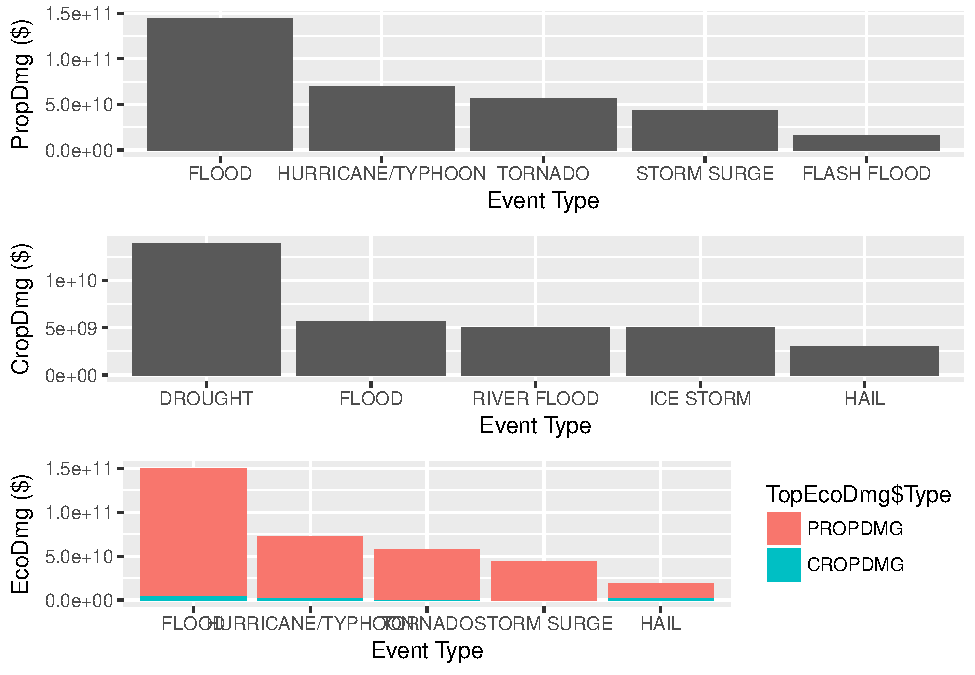
\includegraphics{Project5_4_files/figure-latex/plotEcoDmg-1.pdf}

From the graphs above, we can see Tornado and excessive heat and
lightning are the most harmful events to public health regardless of
which approach we choose. If we prioritise the fatalities then flash
flood and heat are considered as very harmful, otherwise, if we just
consider the sum of fatalities and injuries, tstm wind and flood are
recognised as very harmful instead.

With respect to economy damage caused, flood is the most server event
followed by hurricane/typhoon, tornado, storm surge and hail.


\end{document}
